\chapter{Antecedentes}
\label{chap:antecedentes}

\drop{E}{n} este capítulo se muestra el trabajo de documentación e investigación previa a la realización del presente \ac{TFG}. En primer lugar se abordarán los sistemas de posicionamiento, su historia y el desarrollo del gps\footnote{Debido al extendido uso de la denominación \textit{GPS} como sinónimo de los \ac{GNSS}, se usará de este modo. Para referirse al sistema de posicionamiento propiedad del gobierno de los Estados Unidos \acf{GPS} se utilizará el acrónimo en mayúsculas} 

y los antecedentes de los \ac{SIG}, más tarde se comentarán algunos aspectos relevantes de la web y de las tecnologías móviles. Para terminar, se enumerarán algunas aplicaciones similares que podemos encontrar actualmente en el mercado.

\section{Localización geográfica y \acf{SIG}}

%HISTORIA DEL GPS
Los \ac{GNSS} permiten conocer en tiempo real la posición de un objeto cualquiera en la superficie terrestre.

Según Scott Gleason y Demoz Gebre-Egziabher \cite{Glea09} podríamos definir la navegación como:

	\vspace{5mm}
\begin{tikzpicture}
	\node[shadowBox] {El proceso de determinación de la posición, la velocidad y, en algunos casos, la orientación de un objeto.};
\end{tikzpicture}
	\vspace{5mm}

Por tanto, un \ac{GNSS} consiste en una constelación de satélites que permiten determinar con precisión las coordenadas geográficas y la altitud de un punto dado en cualquier punto de la superficie terrestre.

El inicio de este tipo de sistemas podríamos encontrarlo en los primeros marinos. La decisión de alejarse de las rutas que transcurrían a lo largo de la línea de visión de la costa, con la intención de reducir el tiempo, los costes derivados de los viajes y la posibilidad de encontrar nuevos mercados, planteó un nuevo reto tecnológico consistente en conocer con exactitud la localización en la que se encontraban.
La primera solución vino de la mano de un gran conocimiento de la bóveda celeste y la posición de las estrellas. Usando instrumentos como el astrolabio y el sextante (ver figura \ref{fig:sextante_astrolabio}), se podía calcular con asombrosa exactitud la posición.

\begin{figure}[hbtp]
	\begin{adjustbox}{minipage=\linewidth, fbox}
		\centering
		\subfigure[Sextante]{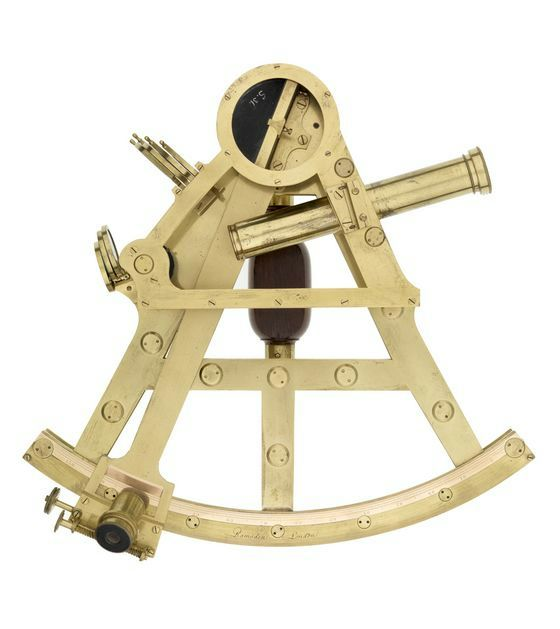
\includegraphics[width=60mm, height=80mm]{./images/03-antecedentes/04-sextante.png}}
		\hspace{10mm}
		\subfigure[Astrolabio]{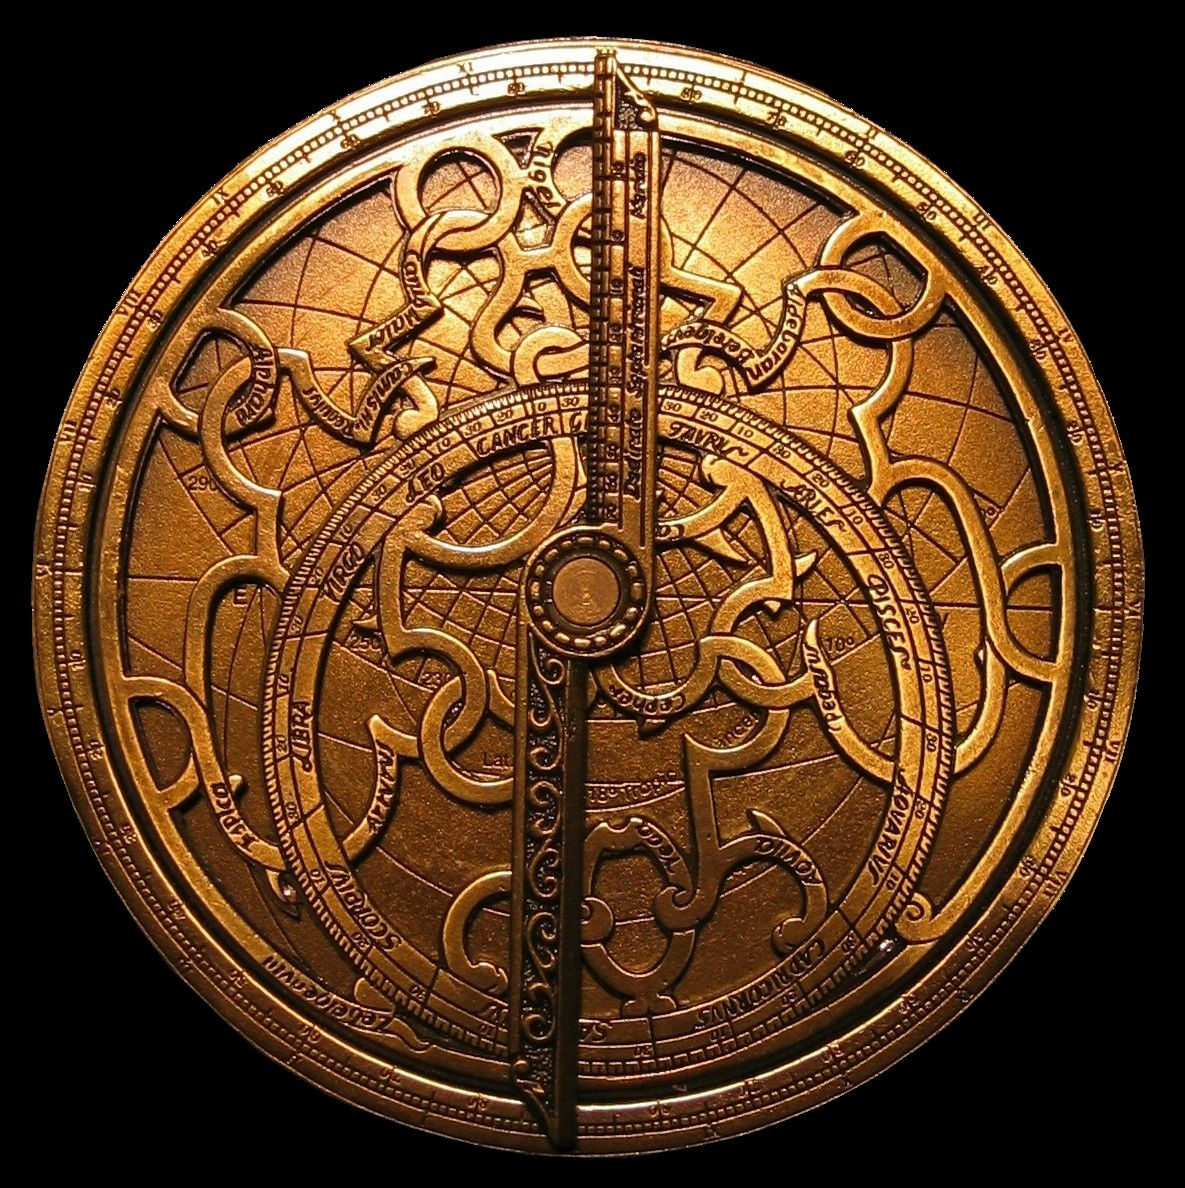
\includegraphics[height=80mm]{./images/03-antecedentes/05-astrolabio.png}}
	\end{adjustbox}
	\caption{Primeros instrumentos de navegación}
	\label{fig:sextante_astrolabio}
\end{figure}

Hasta tiempos recientes (segunda mitad del S. XX), con la irrupción del posicionamiento satelital, este era el método usado para conocer la ubicación en la que se encontraban.
Los primeros prototipos del gps se desarrollan a principios del S. XX, coincidiendo con los comienzos de la automoción, aspecto este último que ha dado la gran fama a esta tecnología.
El primer gps data de 1909, que consistía en un odómetro que giraba un mapa indicando los hitos más importantes que se podían encontrar en el punto kilométrico en el que estabas.
Este primer prototipo se llamaba \textit{Jones Live Map} (ver figura \ref{fig:jones_live_map}), cada mapa era válido para unos 160 km y después había que cambiarlo por el siguiente mapa. Este primer intento dejó de fabricarse en los años 20, cuando las carreteras estaban correctamente señalizadas \cite{GPS12}.

\begin{figure}[hbtp]
\centering
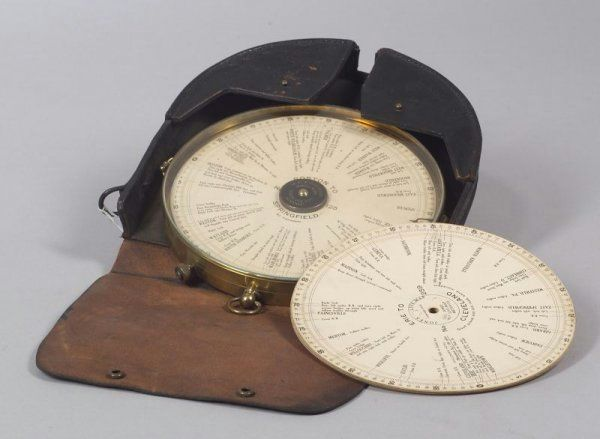
\includegraphics[scale=0.5, fbox={\fboxrule} 4mm]{images/03-antecedentes/06-jones_live_map.png}
\caption{Jones Live Map}
\label{fig:jones_live_map}
\end{figure}

También en la década de los veinte, hizo su aparición el \textit{Plus Fours Routefinder} (ver figura \ref{fig:plus_fours_routefinder}), consistente en un pequeño reloj de muñeca con una serie de papiros con la información de la ruta que debían ir desenrollándose de forma manual para ir viendo las indicaciones \cite{Plus14}.

\begin{figure}[hbtp]
\centering
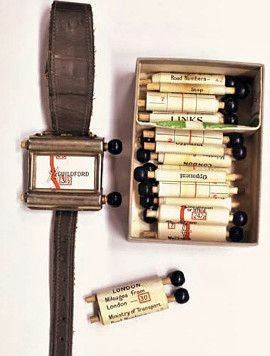
\includegraphics[scale=0.5, fbox={\fboxrule} 4mm]{images/03-antecedentes/07-plus_fours_routefinder.png}
\caption{Plus Fours Routefinder}
\label{fig:plus_fours_routefinder}
\end{figure}

Otro de los padres del gps moderno es el llamado \textit{Iter Avto} (ver figura \ref{fig:iter_avto}), consistente en un mapa enrollado conectado al velocímetro del coche para sincronizarlo. La dos grandes ventajas con respecto al \textit{Plus Fours Routefinder}, consistía en que se instalaba sobre el salpicadero del coche y mostraba de forma gráfica la posición. Su inconveniente, cualquier desviación de la ruta era completamente indetectable \cite{Parra13}.

\begin{figure}[hbtp]
\centering
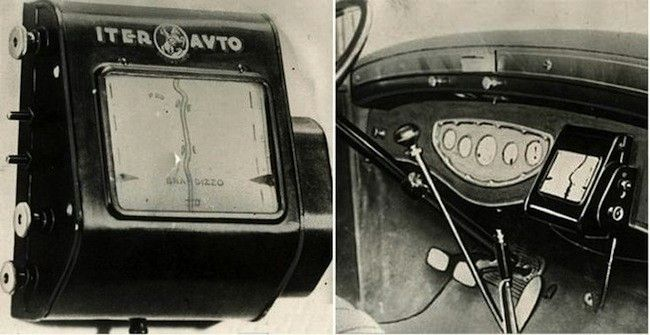
\includegraphics[scale=0.5, fbox={\fboxrule} 4mm]{images/03-antecedentes/08-iter_avto.png}
\caption{Iter Avto}
\label{fig:iter_avto}
\end{figure}

Durante la segunda guerra mundial, la \ac{RAF} desarrolló un sistema de
posicionamiento para sus bombarderos consistente en tres estaciones de radar que localizaban
con precisión al avión \cite{Ori13}.
Los verdaderos orígenes de los gps como sistema de navegación satelital se remontan a 1957 con
el programa \textit{TRANSIT}. Por un lado la marina de los estados unidos inicia el programa \textit{Polaris},
que consiste en el despliegue de misiles transcontinentales suboceánicos. Alcanzar los objetivos
con los misiles dependía de la capacidad de determinar con precisión la posición de los
submarinos en cualquier punto de la superficie terrestre. Por otro lado, la universidad Johns
Hopking de Maryland, consigue determinar con precisión la órbita del \textit{Sputnik 1} a partir del
desplazamiento Doppler sufrido por la señal que emitía y el conocimiento preciso de la posición
del receptor. Con estos elementos, invertir los términos del problema resultó relativamente
sencillo, esto es, conociendo la posición de un satélite de forma precisa, es posible determinar
la de un receptor situado en el submarino de posición desconocida midiendo el desplazamiento
Doppler sufrido por la señal emitida del satélite.

El sistema \textit{TRANSIT} entró en funcionamiento en 1964 con el lanzamiento de 10 satélites y se mantuvo en servicio
hasta 1996. En 1967 se permitió su uso civil. El error típico de este sistema era de unos 250
metros, por lo que resultaba muy útil para la navegación de aviones, barcos y submarinos, pero
por razones obvias (precisión y tamaño de los receptores) aún estaban lejos de los sistemas de
navegación personal actuales.

La Unión Soviética había desarrollado casi al mismo tiempo, un sistema muy parecido con
idénticas prestaciones, el \textit{TSICADA}, lo que resultaba inadmisible para los norteamericanos en el
contexto de la guerra fría, por lo que comenzó a desarrollarse lo que posteriormente sería el
\ac{GPS} \cite{Pala10}.
El \textit{NAVSTAR-GPS} nació en 1973 para uso exclusivamente militar, con una constelación de 24
satélites en órbitas inclinadas de 12 horas, lo que se traducía en que cualquier receptor en el
mundo tendría en su horizonte visible al menos 5 satélites disponibles en todo momento. El
TRANSIT, no sólo no podía garantizar esto, debido a que sus satélites eran de órbita baja, si no
que con sus 6 satélites, algunos receptores podían estar varias horas esperando señal. El primer
satélite se puso en órbita en 1978. La precisión de este nuevo sistema era de 1 metro y podía
ser incorporado en misiles, bombas inteligentes, vehículos, etc. Debido a su consideración de
recurso de gran valor estratégico, su uso estaba limitado al ámbito estrictamente militar.
El 31 de agosto de 1983 tuvo lugar uno de los incidentes internacionales más graves de la
guerra fría, que a la postre resultaría decisivo para el uso actual del \ac{GPS}, el derribo del vuelo de
\textit{Korean Airlines KAL007} por parte de la \ac{URSS} \cite{Kore15}.

El citado vuelo, usando los sistemas de navegación tradicionales disponibles en aquella época, y
usando el piloto automático, invadió en dos ocasiones el espacio aéreo de la Unión Soviética,
que acabó interceptándolo mediante dos cazas militares y derribándole con un ataque con
misiles, matando al pasaje y la tripulación completa, con un resultado de 269 fallecidos.
La respuesta internacional no se hizo esperar, y el entonces presidente de \ac{USA}, Ronald Reagan,
anunció que el sistema \ac{GPS} estaría disponible para propósitos civiles una vez finalizase el
proyecto, con la intención de que no se volvieran a repetir incidentes similares.
Para evitar que sus enemigos pudieran hacer uso de esta nueva tecnología para construir
misiles de precisión con los que atacarlos, el Departamento de Defensa de \ac{EE.UU.} impuso una
serie de restricciones en la precisión de los receptores, de manera que el error en el
posicionamiento fuera mayor que el de los disponibles para uso militar. Por ello los receptores de gps de uso
civil eran incapaces de mostrar una resolución menor de 20 metros.
Durante la primera guerra del golfo, en 1991, se desarrolló una mejora en la precisión del \ac{GPS}
llamada, \ac{GPS} Diferencial, que conseguía precisiones de entre 1 y 3 metros de exactitud.



%HISTORIA DEL SIG
Debido a que el término \ac{SIG} engloba la integración de muy diversas áreas,no existe una única definición totalmente consensuada \cite{Chr97}. La definición aportada por el \ac{NCGIA} resulta ampliamente aceptada:

\vspace{5mm}
\begin{tikzpicture}
	\node[shadowBox] {
	Un SIG es un sistema de hardware, software y procedimientos elaborados para facilitar la obtención, gestión, manipulación, análisis, modelado, representación y salida de datos espacialmente referenciados, para resolver problemas complejos de planificación y gestión.};
\end{tikzpicture}
\vspace{5mm}

Uno de los elementos relevantes de los \ac{SIG} son la asociación de información a una imagen concreta y una de las primeras muestras de esto lo podemos encontrar en el Londres victoriano de mediados del siglo XIX. En el año 1854, el doctor John Snow (ver figura \ref{fig:john_snow}) utilizó un mapa del Soho londinense para ubicar los casos de un brote de cólera (ver figura \ref{fig:cholera_map}). Con la ayuda de los registros del hospital de Middlesex y de Henry Whitehead, párroco local, recogió las defunciones producidas mediante una fina línea de color negro que se apilaban unas sobre otras a medida que se producían las muertes, consiguiendo el efecto de asociación de información a imagen comentado en el párrafo anterior \cite{Cai11}.

Este ejemplo temprano, combinado con la geolocalización nos permite identificar las líneas base de representación de lo que será el presente \ac{TFG}.

\begin{figure}[hbtp]
\centering
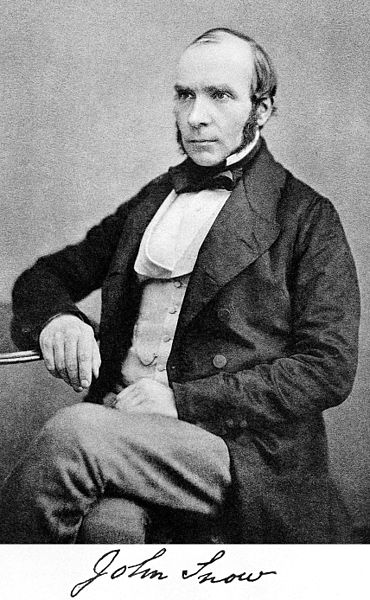
\includegraphics[scale=1, fbox={\fboxrule} 0mm]{images/03-antecedentes/02-john_snow.jpg}
\caption{Doctor Sir John Snow}
\label{fig:john_snow}
\end{figure}

\begin{figure}[hbtp]
\centering
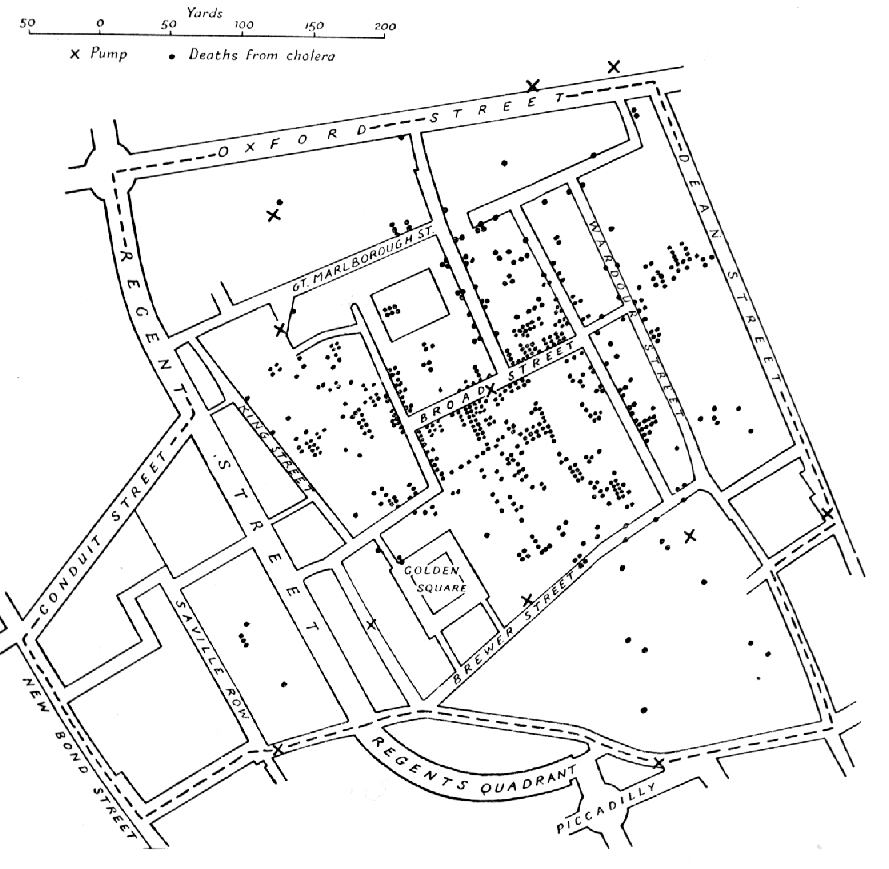
\includegraphics[scale=0.5, fbox={\fboxrule} 4mm]{images/03-antecedentes/01-cholera_map.jpg}
\caption{Mapa del Soho con los casos de fallecimiento por cólera}
\label{fig:cholera_map}
\end{figure}

Gracias a ello y referenciando en el mapa la posición de los pozos de agua, pudo comprobar como una gran cantidad de víctimas se encontraban dentro de la zona de influencia de una bomba de agua en Broad Street (ver figura \ref{fig:cholera_map_detail}), que a la postre resultó estar contaminada con heces. Recomendando la clausura de la misma consiguió acabar con la epidemia      \cite{Gunn07}. Debido a estos logros se le considera el padre de la epidemiología moderna y podemos ilustrar uno de los primeros ejemplos del uso de los \ac{SIG}.

\begin{figure}[hbtp]
\centering
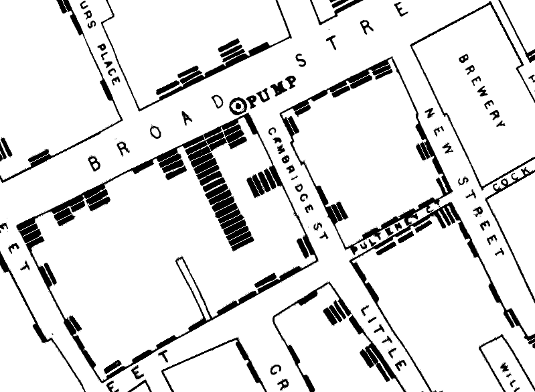
\includegraphics[scale=0.5, fbox={\fboxrule} 4mm]{images/03-antecedentes/03-cholera_map_detail.png}
\caption{Detalle del mapa del Doctor Snow}
\label{fig:cholera_map_detail}
\end{figure}

\section{Internet y la \ac{www}}

%Historia de Internet
Internet puede considerarse como una de las tecnologías que más ha cambiado el mundo y la que más rápidamente lo ha hecho. Gracias a este nuevo concepto, se puede acceder rápidamente a la mayor cantidad de información nunca antes recopilada en la historia de la humanidad.\\

La gran biblioteca de Alejandría, la mayor de las bibliotecas del mundo antiguo, contenía, según Flavio Josefo, antes de su destrucción unos 200.000 volúmenes y consideraban que todo el conocimiento de la humanidad ocuparía un total de 500.000 volúmenes  \cite{Jos94}. Autores modernos han recalculado el posible número de volúmenes, aportando una cifra de unos 50.000 rollos, que podría equivaler a unos 12.500 libros actuales \cite{Esco01}.\\

Los Archivos Secretos Vaticanos contienen un total de 1.600.000 volúmenes \cite{Bav15}, la biblioteca nacional de España 28 millones \cite{Sanz15} y la biblioteca del congreso de los \ac{EE.UU} 160 millones de documentos \cite{Libr15}. Comparando las cifras de algunas de las mayores bibliotecas del mundo con el número de documentos existentes en Internet, podemos hacernos una idea de lo que esta tecnología a supuesto para la humanidad, no solamente en el volumen de información existente, si no en la facilidad de acceso a los mismos. En el año 2012, en Internet existían un total de 8.310 millones de documentos accesibles.

Aunque no es lícito comparar estas cifras en bruto, ya que tal la cantidad no siempre está relacionada con la calidad, como dijo el escritor Neil Gaiman \cite{Gaim10}:

\vspace{5mm}
\begin{tikzpicture}
	\node[shadowBox] {
	Google puede devolverte cien mil respuestas, un bibliotecario puede devolverte la correcta.};
\end{tikzpicture}
\vspace{5mm}

En el año 1958 la compañía Bell crea el primer módem, un dispositivo capaz de transmitir datos binarios utilizando una línea telefónica (ver figura \ref{fig:bell_modem}). En el año 1962 J.C.R Licklider describe su concepto de \textit{Red galáctica}, consistente en una red interconectada globalmente que permitiera acceder a todo tipo de datos y programas desde cualquier sitio. Un año antes, en 1961, Leonard Kleinrock publicó su tesis doctoral acerca de la teoría de colas, que sería publicado como libro en el año 1964 (\cite{Klei64}) y que sirvió de fundamento a la teoría de conmutación de paquetes. Los datos se troceaban en partes, llamadas \textit{paquetes}, a los que se les asignaba un número de secuencia antes de enviarlos. De esta manera, no importaba en orden en que llegasen al receptor, puesto que podría recomponer el mensaje original.
En el año 1967 en una conferencia, se presentaba el proyecto inicial de \ac{ARPANET}. Durante las discusiones iniciales del proyecto se llegó a la conclusión de desligar la comunicación de la máquina principal, crean pequeños computadores que fuesen quienes cargasen con la responsabilidad de lidiar con las líneas telefónicas. El 29 de Octubre de 1969 se transmite el primer mensaje a través de \ac{ARPANET} y el 21 de Noviembre de ese mismo año se establece la primera conexión entre las computadoras de la universidad de Stanford y \ac{UCLA}. 

\begin{figure}[hbtp]
\centering
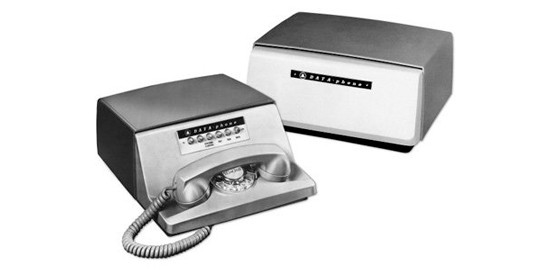
\includegraphics[scale=0.5, fbox={\fboxrule} 4mm]{images/03-antecedentes/09-modem_bell.jpg}
\caption{Módem Bell. 1958}
\label{fig:bell_modem}
\end{figure}

En el año 1972 al calor de una grande y exitosa demostración de \ac{ARPANET}, se introduce la primera gran aplicación de esta nueva tecnología, el correo electrónico. Ray Tomlinson, había desarrollado para \ac{ARPANET} unos años antes un programa llamado SNDMSG para enviar mensajes entre las distintas terminales de una computadora, por lo que adaptó este programa para permitir el envío dentro de una red más amplia.

Con el crecimiento de la red, se desarrollaron tres protocolos que actualmente siguen en uso, \ac{TCP}, \ac{IP} y \ac{DNS}. El año 1983, \ac{ARPANET} se abre definitivamente a la vida civil permitiendo el intercambio masivo de datos entre universidades y centros de investigación. Este es el motivo último por el que se celebra ese año como el nacimiento de Internet.

La \textit{web} (\ac{www}) es probablemente el punto más visible de Internet. Fue desarrollado entre 1989 y 1990 por Tim Berners-Lee y Robert Cailiau mientras trabajaban en el \ac{CERN}.

En la web, es utilizado \ac{HTTP} como protocolo de comunicación, que define la sintaxis y la semántica necesarias para el correcto funcionamiento de los distintos componentes de la comunicación web, consiguiendo una abstracción que permite unificar la forma de comunicación en la red. En las comunicaciones en red el modelo de arquitectura más extendido es el paradigma Cliente - Servidor (ver figura \ref{fig:cliente-servidor}), mediante el cual se define una máquina \textit{servidor} encargada de generar la corriente datos y una serie de máquinas conocidas como \textit{clientes}, que realizan peticiones para consumir estos datos. El funcionamiento básico de este modelo podría verse como una farmacia abierta 24 horas (servidor), que está permanentemente a la espera de que alguna persona decida entrar a comprar algún medicamento, momento en el cual busca la droga pedida y se la facilita.

\begin{figure}[hbtp]
\centering
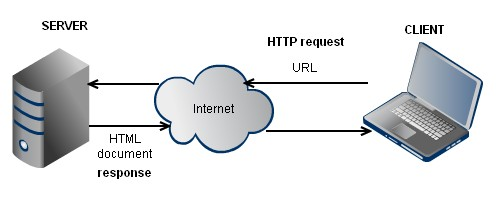
\includegraphics[scale=0.5, fbox={\fboxrule} 4mm]{images/03-antecedentes/10-client_server.png}
\caption{Modelo cliente-servidor}
\label{fig:cliente-servidor}
\end{figure}

Para que estas transacciones puedan darse, los computadores deben poder conocer como comunicarse, lo que en este caso se logra mediante las direcciones\ac{IP}, una serie de 32 bits que designan unívocamente un elemento de una red, y unos pocos pasos intermedios, y transparentes, para el usuario. El cliente, normalmente mediante un navegador web, es decir, mediante un programa creado específicamente para la navegación y visualización de páginas web, introduce el nombre de la página web con la que quiere comunicarse. Este nombre, por ejemplo, \textit{www.usipv6.com}, es enviado automáticamente a unos servidores llamados \ac{DNS}, que son capaces de buscar la dirección \ac{IP} asociada al nombre de la página tecleada y devolver su dirección \ac{IP}, que en este caso podría ser \textit{123.45.67.89} (ver figura \ref{fig:dns-server}). Es fácil ver el porque se utiliza este paso intermedio, debido a que al usuario le resultará mucho más sencillo recordar una página web que una serie de números. Una vez realizada la traducción, el computador se comunica con el servidor a través de la dirección \ac{IP} obtenida y este le responde enviándole la información solicitada.

\begin{figure}[hbtp]
\centering
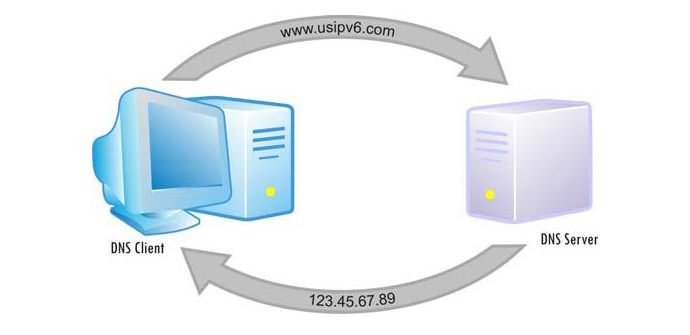
\includegraphics[scale=0.5, fbox={\fboxrule} 4mm]{images/03-antecedentes/11-dns_server.png}
\caption{Comunicación con servidor DNS}
\label{fig:dns-server}
\end{figure}

Aunque en sus orígenes,la web se desarrolló para transmitir únicamente texto, actualmente, como es fácil ver, se permite la emisión de todo tipo de contenidos multimedia, como audio, vídeo o imágenes. La tarea del cliente, consiste en recibir los datos enviados por el emisor y reinterpretarlos y mostrarlos de manera coherente para el usuario.

Todo esto nos lleva a poder diferenciar claramente dos trabajos distintos dentro de la comunicación web, el trabajo llevado a cabo por el cliente y el trabajo llevado a cabo por el servidor. Para poder desarrollar cada una de estas tareas, existen una serie de tecnologías específicas para el lado del cliente y para el lado del servidor.

\subsection{Tecnologías del lado del servidor}
Como se ha explicado en la sección anterior, el servidor es el encargado de atender las peticiones que los clientes le envían y responderlas adecuadamente. 
En los comienzos de la web los servidores eran meras estaciones de \textit{almacenaje}, que devolvía al cliente peticionario una página web estática (ver figura \ref{fig:static-server}) mientras que en la actualidad, los servidores son capaces de generar el contenido a enviar de forma dinámica (ver figura \ref{fig:dynamic-server}).

\begin{figure}[hbtp]
\centering
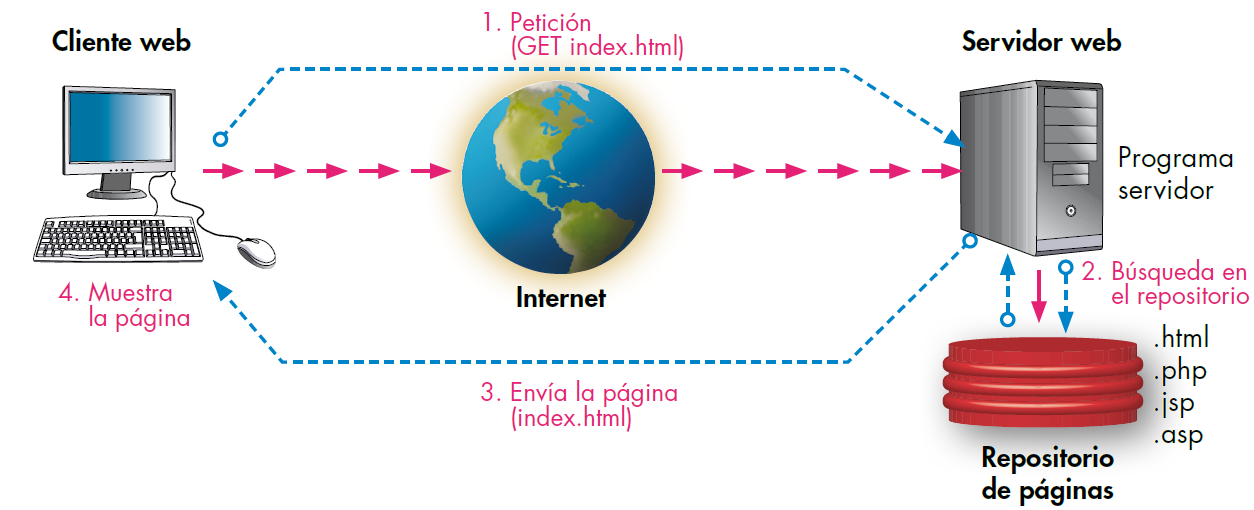
\includegraphics[scale=0.5, fbox={\fboxrule} 4mm]{images/03-antecedentes/12-html_request.png}
\caption{Petición a servidor estático}
\label{fig:static-server}
\end{figure}

\begin{figure}[hbtp]
\centering
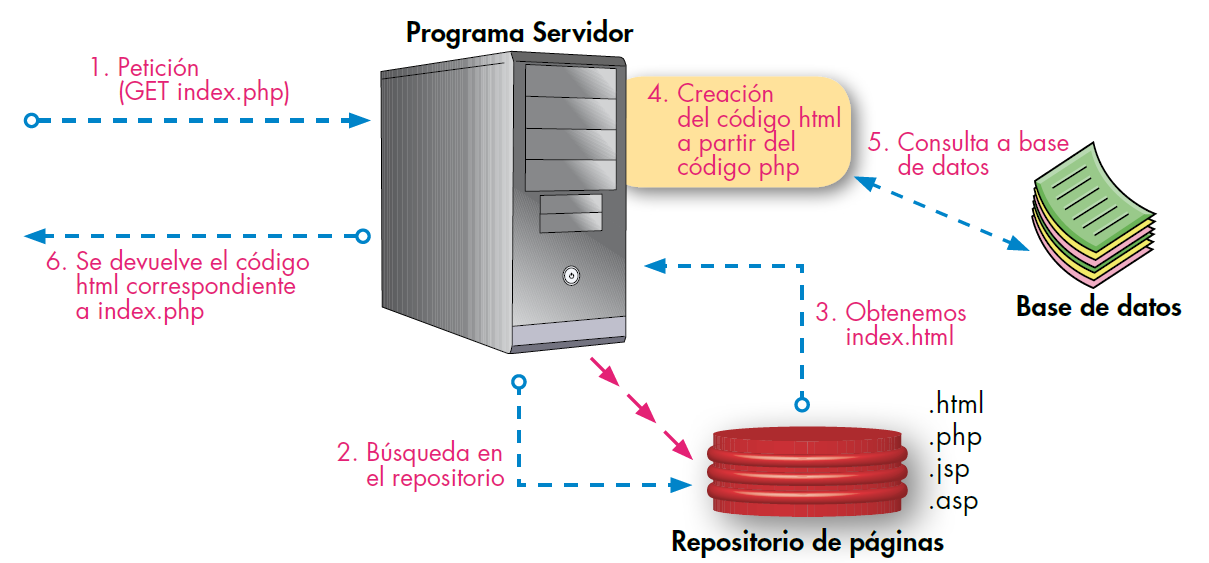
\includegraphics[scale=0.5, fbox={\fboxrule} 4mm]{images/03-antecedentes/13-html_dynamic_request.png}
\caption{Petición a servidor dinámico}
\label{fig:dynamic-server}
\end{figure}

Algunas de las tecnologías más utilizadas en el lado del cliente son Apache, PHP y MySQL.

Apache es un software que permite a un computador realizar un comportamiento de servidor, esto es, atender a las peticiones de los clientes, ofrecerles servicios y enviarles la información pedida. Esta desarrollado en C y es de código abierto \cite{Apac15}.

PHP es uno de los lenguaje de programación del lado del servidor más extendido y fue uno de los primeros en poder ser incorporado directamente en el código \ac{HTTP}. Fue creado por Rasmus Lerdorf en 1994 y actualmente se encuentra en su versión 5.6.14 \cite{Hist15}.

MySql es un sistema de gestión de bases de datos relacionales desarrollado por MySQL AB (actualmente parte de Sun Microsystems) en 1995 por Michael Widenius, David Axmark and Allan Larsson \cite{Data14}.

\begin{figure}[hbtp]
	\begin{adjustbox}{minipage=\linewidth, fbox}
		\centering
		\subfigure[MySQL]{
\includegraphics[scale=0.75]{./images/03-antecedentes/14-mysql.png}}
		\hspace{10mm}
		\subfigure[PHP]{
\includegraphics[scale=0.75]{./images/03-antecedentes/15-php.png}}
		\vspace{10mm}
		\subfigure[Apache]{
\includegraphics[scale=0.75]{./images/03-antecedentes/16-apache.png}}
	\end{adjustbox}
	\caption{Tecnologías utilizadas en servidores}
	\label{fig:mysql_php_apache}
\end{figure}

\subsection{Tecnologías del lado del cliente}
Dejando de lado la necesidad de contar con un navegador web que permita mostrar e interactuar con las páginas web mostradas, el cliente debe interpretar los datos recibidos por el servidor de manera que pueda traducirlos convirtiéndolos en el concepto de \textit{página web} que conocemos. Tres de los lenguajes más utilizados en este intercambio de datos son \ac{HTML}, \ac{CSS}, JavaScript y \ac{AJAX}.

\ac{HTML} es un lenguaje de marcado que se utiliza para la representación visual de una página web. Está considerado el lenguaje de programación más importante y está a cargo de la W3C \cite{Worl15}. Aunque permite dar formato al texto, actualmente esto suele ser responsabilidad de las hojas \ac{CSS}.

La última versión, \ac{HTML}5, publicada en octubre de 2014 \cite{Adam14} incorpora novedades como etiquetas con codecs, para manejar grandes conjuntos de datos o mejoras en los formularios.

\ac{CSS} es usado para definir el formato de una página web escrita en \ac{HTML}.

\begin{lstlisting}[
  float=ht,
  language = HTML,
  caption  = {«Hola mundo» en HTML y CSS},
  label    = code:hello]
	<!DOCTYPE html>
	<html>
	<head>
	    <title>Hola Mundo en HTML</title>
		<style>
		body {background-color:lightgrey}
		h1   {color:blue}
		p    {color:green}
		</style>
	</head>
	<body>
		<h1>Hola Mundo</h1>
		<p>Mi primera web en HTML y CSS.</p>
	</body>
	</html>
\end{lstlisting}

Javascript es un lenguaje interpretado orientado a objetos implementado normalmente como parte del navegador web.
\ac{AJAX} es utilizado para poder realizar peticiones a un servidor modificando partes concretas de una página, eliminando de esta forma la necesidad de recargar la página completa.

% Desarrollo web (frameworks)


\section{Dispositivos móviles}
Lo teléfonos móviles han cambiado nuestra manera de relacionarnos tanto con el mundo como entre las personas. No hace más de diez años era imposible pensar en poder acceder a Internet desde cualquier lugar o tener la posibilidad de enviar mensajes a través de 
las aplicaciones de mensajería instantánea. Hace veinte o treinta años nadie imaginaba que los teléfonos móviles serían un elemento imprescindible y omnipresente de nuestras vidas ya que en aquella época era símbolo de estatus y gran lujo.

Podríamos comenzar a explicar los intentos de comunicarse a través de grandes distancias con el telégrafo, primer gran antecedente del teléfono, y es que este invento fue algo revolucionario cuando se presentó. Por primera vez se podían comunicar dos puntos distantes de manera instantánea.

Los orígenes del telégrafo se remontan al S. XVIII cuando Claude Chappe desarrolló para el ejército Francés su precursor inmediato, el telégrafo óptico. Este invento consistía en un sistema de comunicación que emitía una señal visual que podía repetirse en la distancia, aunque solo tenía utilidad en las distancias a las que el ojo pudiera abarcar \cite{Holz94}.

\begin{figure}[hbtp]
	\begin{adjustbox}{minipage=\linewidth, fbox}
		\centering
		\subfigure[Telégrafo óptico de Claude Chappe]{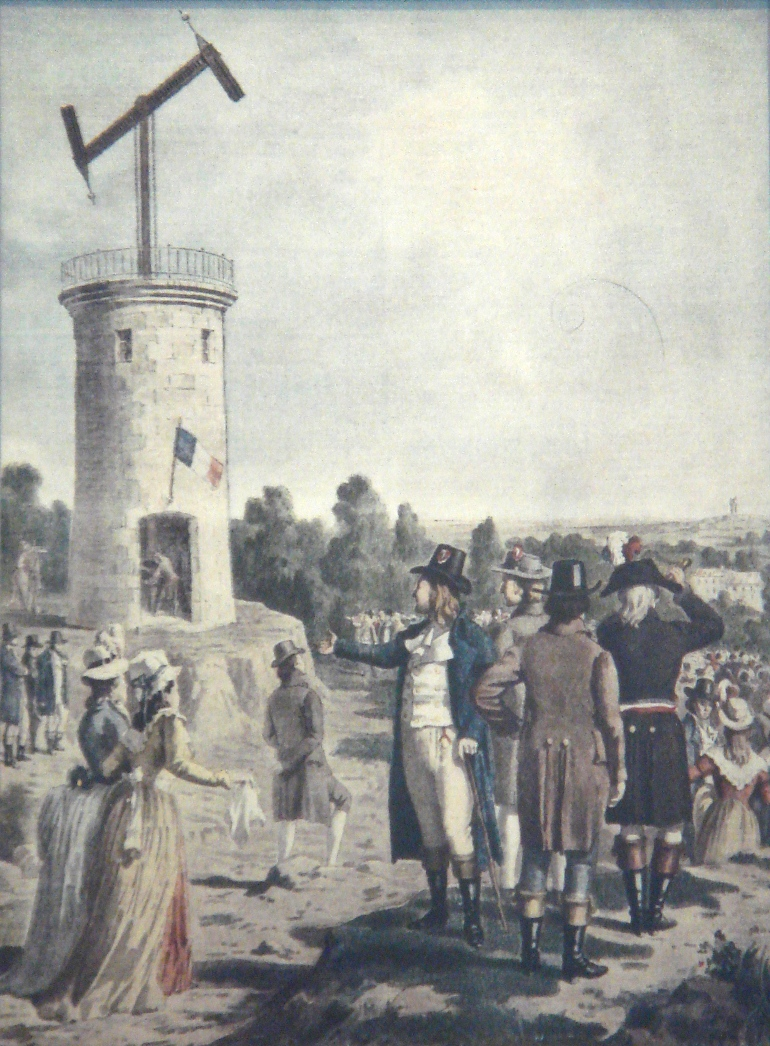
\includegraphics[height=80mm]{./images/03-antecedentes/17-telegrafo_optico.jpg}}
		\hspace{10mm}
		\subfigure[Claude Chappe]{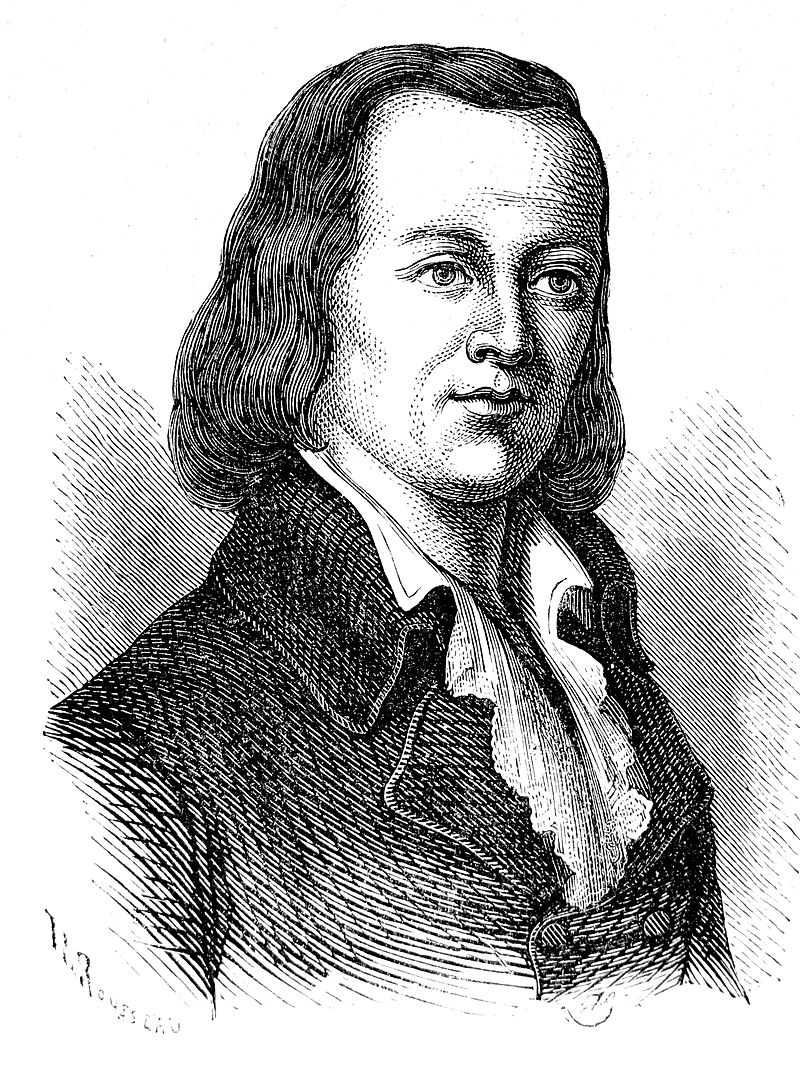
\includegraphics[height=80mm]{./images/03-antecedentes/18-claude_chappe.jpg}}
	\end{adjustbox}
\caption{Telégrafo óptico}
	\label{fig:telegrafo_optico}
\end{figure}

Con la intención de mejorar el alcance de la comunicación y aprovechando los estudios de electromagnetismo de Michael Faraday y las innovaciones de William Sturgeon y Joseph Henry sobre el electroimán, Samuel Morse (ver figura \ref{fig:telegrafo}) ideó una manera de enviar señales entre dos puntos aprovechando las corrientes eléctricas. En un primer momento, el telégrafo consistía en un péndulo que ante la existencia de corriente movía un lápiz que dibujaba de esa manera una línea sobre un papel. Mejorando el prototipo se llego a inventar el famoso código morse, que consta de los consabidos dos elementos: el punto y la raya.

\begin{figure}[hbtp]
	\begin{adjustbox}{minipage=\linewidth, fbox}
		\centering
		\subfigure[Samuel Morse]{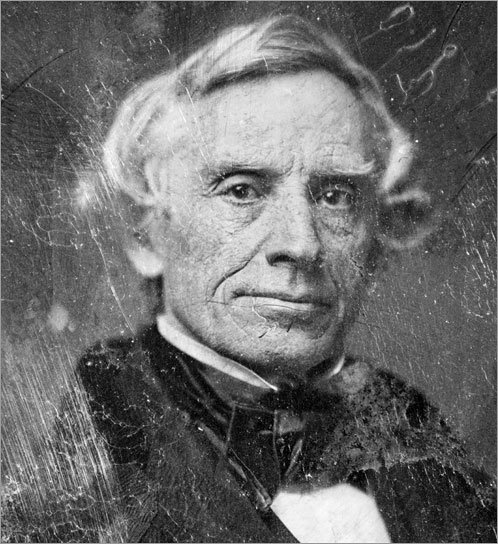
\includegraphics[height=80mm]{./images/03-antecedentes/20-samuel_morse.jpg}}
		\hspace{10mm}
		\subfigure[Código morse]{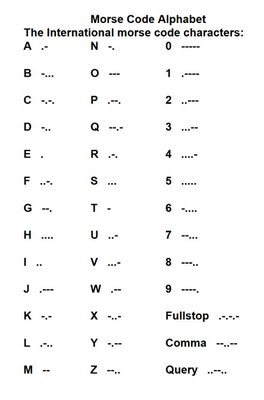
\includegraphics[height=80mm]{./images/03-antecedentes/21-codigo_morse.jpg}}
	\end{adjustbox}
\caption{Telégrafo}
	\label{fig:telegrafo}
\end{figure}

En 1837 Samuel Morse hizo la primera demostración pública del telégrafo en un áula de la universidad de Nueva York. La gran aportación de Morse.

El 24 de mayo de 1844, se terminó la línea que unía Baltimore y Washington, enviando un mensaje desde la Cámara de Corte Suprema de en el Capitolio de \ac{EE.UU.} en Washington hasta el ferrocarril B \& O en Baltimore con la frase \textit{What hath God wrought?} perteneciente al libro de los Números (ver figura \ref{fig:telegrama}).

\begin{figure}[hbtp]
\centering
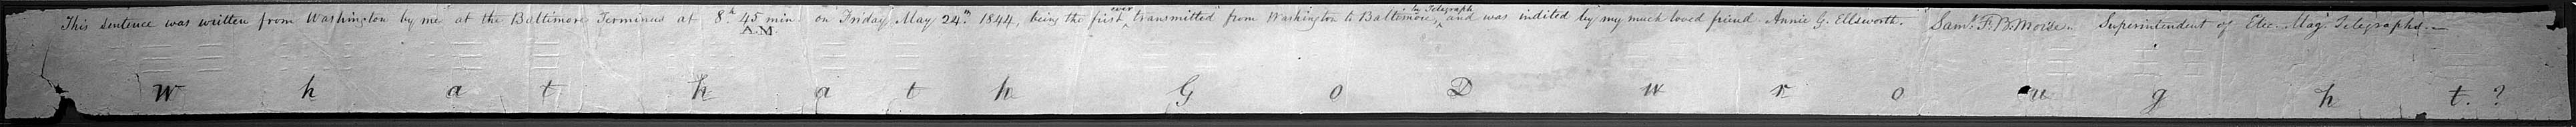
\includegraphics[width=100mm, fbox={\fboxrule} 4mm]{images/03-antecedentes/19-primer_telegrama.jpg}
\caption{Primer telegrama}
\label{fig:telegrama}
\end{figure}

El siguiente gran paso en las comunicaciones viene de la mano de un dispositivo capaz de retransmitir, a través de cables, las señales acústicas derivadas de la voz humana. El teléfono.

Históricamente, la invención del teléfono se atribuyó a Alexander Graham Bell \cite{Cab79}, aunque el 11 de junio de 2002 fue reconocido el italiano Antonio Meucci (ver figura \ref{fig:teléfono}) como el verdader inventor de este aparato por el Congreso de los Estados Unidos \cite{Uni03}.

\begin{figure}[hbtp]
	\begin{adjustbox}{minipage=\linewidth, fbox}
		\centering
		\subfigure[Antonio Meucci]{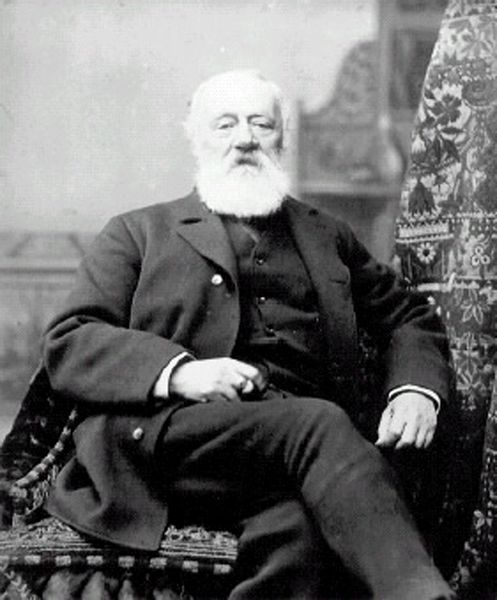
\includegraphics[height=80mm]{./images/03-antecedentes/22-antonio_meucci.jpg}}
		\hspace{10mm}
		\subfigure[Alexander Graham Bell]{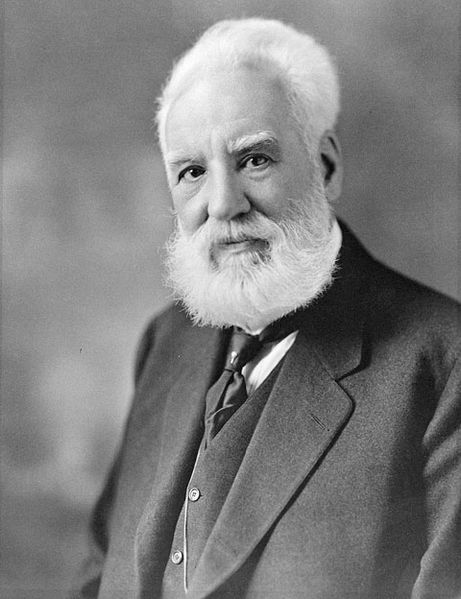
\includegraphics[height=80mm]{./images/03-antecedentes/23-alexander_graham_bell.jpg}}
	\end{adjustbox}
\caption{Inventores del teléfono}
	\label{fig:teléfono}
\end{figure}

Antonio Meucci, nacido en Florencia, emigró junto a su esposa Ester Mochi primero a Cuba en octubre de 1835 y después a Staten Island, Nueva York \ac{EE.UU.} en 1850.

\section{Aplicaciones similares}



% Local Variables:
%  coding: utf-8
%  mode: latex
%  mode: flyspell
%  ispell-local-dictionary: "castellano8"
% End:
